\documentclass[border=10pt]{standalone}
\usepackage{tikz}\usepackage{amsmath}\usetikzlibrary{arrows.meta}
\begin{document}
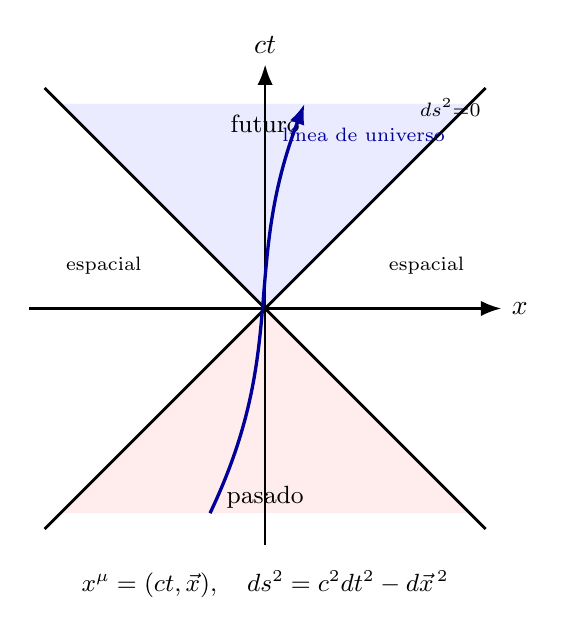
\begin{tikzpicture}[line width=0.9pt,>={Latex[length=2.6mm]}]
  \fill[blue!8] (0,0)--(-2.6,2.6)--(2.6,2.6)--cycle;
  \fill[red!7] (0,0)--(-2.6,-2.6)--(2.6,-2.6)--cycle;
  \draw[->] (-3,0)--(3,0) node[right]{$x$};
  \draw[->] (0,-3)--(0,3.1) node[above]{$ct$};
  \draw[line width=1pt] (-2.8,-2.8)--(2.8,2.8);
  \draw[line width=1pt] (-2.8,2.8)--(2.8,-2.8);
  \node at (0,2.35){\small futuro};
  \node at (0,-2.4){\small pasado};
  \node at (2.05,0.55){\scriptsize espacial};
  \node at (-2.05,0.55){\scriptsize espacial};
  % linea de universo temporal
  \draw[->,blue!60!black,line width=1.2pt] (-0.7,-2.6) .. controls (0.3,-0.5) and (-0.3,0.5) .. (0.5,2.6);
  \node[blue!60!black] at (1.25,2.2){\scriptsize línea de universo};
  \node at (2.35,2.55){\scriptsize $ds^2{=}0$};
  \node[align=center] at (0,-3.5){\small $x^\mu=(ct,\vec x),\quad ds^2=c^2dt^2-d\vec x^{\,2}$};
\end{tikzpicture}
\end{document}
